\documentclass{beamer}

\usepackage{Archivo}
\renewcommand{\sfdefault}{\rmdefault}
\usepackage{graphicx}
\usepackage{tikz}
\usetikzlibrary{calc}
\usepackage[most]{tcolorbox}

%% ---- Superteam Poland brand colors ----
\definecolor{stpldark}{HTML}{0B0E0F}   % near-black background
\definecolor{stplcard}{HTML}{161A1B}   % card / block surface
\definecolor{stplborder}{HTML}{1E2526}  % subtle track color for progress bar
\definecolor{stplred}{HTML}{DC143C}    % brand crimson red
\definecolor{stplwhite}{HTML}{FFFFFF}  % white
\definecolor{stplmuted}{HTML}{8A9BA8}  % muted / secondary text

\usetheme{default}
\setbeamersize{text margin left=0.85cm, text margin right=0.85cm}

%% ---- Background & base text ----
\setbeamercolor{background canvas}{bg=stpldark}
\setbeamercolor{normal text}{fg=stplwhite, bg=stpldark}
\usebeamercolor{normal text}

%% ---- Background image helpers ----
\newcommand{\stpldefaultbg}{%
  \setbeamertemplate{background}{%
    \begin{tikzpicture}[remember picture, overlay]
      \node[at=(current page.center), inner sep=0pt] {%
        
\includegraphics[width=\paperwidth,height=\paperheight]{images/bg-default.png}%
      };
      \fill[stplborder]
        (current page.north west) rectangle
        ([yshift=-2.5pt]current page.north east);
      \pgfmathsetmacro{\stplprog}{\insertframenumber/\inserttotalframenumber}
      \fill[stplred]
        (current page.north west) rectangle
        ($(current page.north west)+(\stplprog\paperwidth,-2.5pt)$);
    \end{tikzpicture}%
  }%
}
\newcommand{\stplherobg}{%
  \setbeamertemplate{background}{%
    
\includegraphics[width=\paperwidth,height=\paperheight]{images/bg-hero.png}%
  }%
}
\stpldefaultbg

%% ---- Structure ----
\setbeamercolor{structure}{fg=stplred}

%% ---- Title slide metadata ----
\setbeamercolor{title}{fg=stplwhite}
\setbeamercolor{subtitle}{fg=stplred}
\setbeamercolor{author}{fg=stplwhite}
\setbeamercolor{institute}{fg=stplmuted}
\setbeamercolor{date}{fg=stplmuted}

%% ---- Frame title: flat, no box background ----
\setbeamercolor{frametitle}{fg=stplwhite, bg=}
\setbeamerfont{frametitle}{size=\large, series=\bfseries}
\setbeamertemplate{frametitle}{%
  \vspace{0.35cm}%
  {\centering\insertframetitle\par}%
  \nointerlineskip\vspace{0.18cm}%
  \hfil{\color{stplred}\rule{2.2cm}{1.5pt}}\hfil\par%
}



%% ---- Incremental reveals ----
\beamerdefaultoverlayspecification{<+->}

%% ---- Bullet items ----
\setbeamercolor{itemize item}{fg=stplred}
\setbeamercolor{itemize subitem}{fg=stplmuted}
\setbeamercolor{itemize subsubitem}{fg=stplmuted}
\setbeamertemplate{itemize item}{\bfseries\textendash}
\setbeamertemplate{itemize subitem}{\small\textendash}
\setbeamercolor{enumerate item}{fg=stplred}
\setbeamercolor{enumerate subitem}{fg=stplmuted}

%% ---- Blocks (flat left-accent via tcolorbox) ----
\tcbset{
  stplbase/.style={
    enhanced, breakable,
    colback=stplcard, coltext=stplwhite,
    coltitle=stplwhite, fonttitle=\bfseries,
    boxrule=0pt, leftrule=3pt,
    arc=0pt, outer arc=0pt,
    top=5pt, bottom=5pt, left=7pt, right=7pt,
    toptitle=4pt, bottomtitle=4pt,
    titlerule=0pt,
  },
}
\renewenvironment{block}[1]{%
  \begin{tcolorbox}[stplbase, colframe=stplred, title={#1}]%
}{%
  \end{tcolorbox}%
}
\renewenvironment{alertblock}[1]{%
  \begin{tcolorbox}[stplbase, colframe=stplred!75!black,
    colback=stplred!10!stplcard, title={#1}]%
}{%
  \end{tcolorbox}%
}
\renewenvironment{exampleblock}[1]{%
  \begin{tcolorbox}[stplbase, colframe=stplmuted, title={#1}]%
}{%
  \end{tcolorbox}%
}

%% ---- Table of contents ----
\setbeamercolor{section in toc}{fg=stplwhite}
\setbeamercolor{subsection in toc}{fg=stplmuted}
\setbeamertemplate{section in toc}{%
  {\color{stplred}\textbf{\textendash}}\hspace{0.5em}\inserttocsection%
}

%% ---- Footline: minimal ----
\setbeamertemplate{footline}{%
  \begin{beamercolorbox}[wd=\paperwidth, ht=0pt, dp=0.55cm]{normal text}%
    \hspace{0.85cm}%
    
\includegraphics[height=1.6ex]{images/stpl-logo.png}%
    \hfill%
    \textcolor{stplmuted}{\tiny\insertframenumber\,/\,\inserttotalframenumber}%
    \hspace{0.85cm}%
  \end{beamercolorbox}%
}
\setbeamertemplate{navigation symbols}{}

%% ---- Title frame helper (uses hero background) ----
\newcommand{\maketitleframe}{%
  \stplherobg
  \begin{frame}[plain]%
    \titlepage%
  \end{frame}%
  \stpldefaultbg
}

%% ---- Section divider slides ----
\AtBeginSection[]{%
  \stplherobg
  \begin{frame}[plain]
    \begin{tikzpicture}[remember picture, overlay]
      \fill[stplred, opacity=0.07]
        ([xshift=-2.5cm]current page.east) circle (5.5cm);
      \fill[stplred]
        (current page.north west) rectangle ([xshift=5pt]current page.south west);
    \end{tikzpicture}%
    \vfill
    \hspace{0.1\paperwidth}%
    \begin{minipage}{0.8\paperwidth}
      \textcolor{stplmuted}{\small Section \thesection}\\[0.35cm]
      {\color{stplwhite}\LARGE\bfseries\insertsectionhead}\\[0.25cm]
      {\color{stplred}\rule{3cm}{1.5pt}}
    \end{minipage}%
    \vfill
  \end{frame}%
  \stpldefaultbg
}

%% ---- Title page ----
\setbeamertemplate{title page}{%
  \begin{tikzpicture}[remember picture, overlay]
    \fill[stplred]
      (current page.north west) rectangle ([xshift=5pt]current page.south west);
    \fill[stplred, opacity=0.07]
      ([xshift=-3cm,yshift=3cm]current page.north east) circle (5.5cm);
    \fill[stplred, opacity=0.04]
      ([yshift=-1.5cm]current page.south east) circle (3.5cm);
  \end{tikzpicture}%
  \vfill
  \hspace{0.08\paperwidth}%
  \begin{minipage}{0.85\paperwidth}
    
\includegraphics[width=3cm]{images/stpl-logo.png}\par
    \vspace{0.8cm}
    {\usebeamerfont{title}\usebeamercolor[fg]{title}\inserttitle}\par
    \vspace{0.2cm}
    {\color{stplred}\rule{3cm}{1.5pt}}\par
    \vspace{0.3cm}
    {\usebeamerfont{subtitle}\usebeamercolor[fg]{subtitle}\insertsubtitle}\par
    \vspace{0.65cm}
    {\usebeamerfont{author}\usebeamercolor[fg]{author}\insertauthor}\par
    \vspace{0.12cm}
    {\small\textcolor{stplmuted}{\insertinstitute\enspace·\enspace\insertdate}}
  \end{minipage}%
  \vfill
}


\usepackage[utf8]{inputenc}
\usepackage[T1]{fontenc}
\usepackage{amsmath}

\title{AMM na Solanie}
\subtitle{Wymiana tokenów bez giełdy --- Solana Bootcamp}
\author{}
\institute{Superteam Poland}

\begin{document}

\maketitleframe

\begin{frame}{Plan}
  \tableofcontents
\end{frame}

% ================================================================
\section{Czym jest DeFi?}

\begin{frame}{Wracamy do obietnicy}
  \begin{itemize}
    \item Lekcja 0 obiecała usługi finansowe \textbf{bez pośrednika}
    \item Bank, broker, notariusz znikają --- ich rolę przejmuje kod
    \item Dwa filary, którymi zbudujemy ten brak pośrednika: \textbf{wymiana tokenów} i \textbf{pożyczki}
    \item Ta lekcja --- wymiana. Pożyczki w następnej.
  \end{itemize}
  \vspace{0.25cm}
  \begin{alertblock}{Jak bez pośrednika?}
    Każdy ruch wymaga zgody na stan rachunku. Skoro nikt go nie pilnuje ---
    co go pilnuje?
  \end{alertblock}
\end{frame}

\begin{frame}{Czym jest DeFi?}
  \begin{itemize}
    \item \textbf{Decentralized Finance (DeFi)} --- usługi finansowe bez pośredników
    \item Program on-chain zamiast banku lub brokera
    \item Permissionless --- każdy może korzystać, bez KYC
    \item Composable --- protokoły łączą się jak klocki
  \end{itemize}
  \vspace{0.3cm}
  \begin{exampleblock}{Dwa przykłady}
    Wymieniasz 100 USDC na SOL w kilka sekund --- bez konta na giełdzie. \\
    Wpłacasz tokeny i zarabiasz odsetki --- bez banku.
  \end{exampleblock}
\end{frame}

\begin{frame}{Token to saldo z regułami}
  \begin{itemize}
    \item Złoty czy dolar wymagają banku, który prowadzi rejestr posiadaczy
    \item Solana zna jeden mechanizm zapisu wartości --- konto z saldem
    \item Saldo bez banku, z regułami zaszytymi w kodzie --- to \textbf{token}
    \item Token może oznaczać walutę, udział w puli, głos albo bilet wstępu
  \end{itemize}
  \vspace{0.25cm}
  \begin{exampleblock}{Analogia --- żeton w kasynie}
    Żeton ma wartość tylko w danym kasynie. Reguły wymiany zna kasyno,
    nie bank. Token on-chain działa tak samo, tylko kasynem jest kod.
  \end{exampleblock}
\end{frame}

% ================================================================
\section{AMM --- Automated Market Maker}

\begin{frame}{Order book vs AMM}
  \begin{columns}
    \column{0.48\textwidth}
      \begin{block}{Order Book (CEX)}
        \begin{itemize}
          \item Kupujący i sprzedający składają zlecenia
          \item Cena wynika z dopasowania zleceń
          \item Wymaga animatorów rynku (market makers)
          \item Przykład: Binance, Openbook
        \end{itemize}
      \end{block}

    \column{0.48\textwidth}
      \begin{block}{\textbf{Automated Market Maker (AMM)}}
        \begin{itemize}
          \item Brak zleceń --- cena z formuły matematycznej
          \item Płynność dostarcza każdy (LP)
          \item Swap zawsze możliwy, 24/7
          \item Przykład: Orca, Raydium
        \end{itemize}
      \end{block}
  \end{columns}
\end{frame}

\begin{frame}{Jak działa AMM}
  \begin{center}
    \begin{tikzpicture}[
        every node/.style={font=\scriptsize\bfseries},
        box/.style={
          draw=stplred, line width=1pt,
          fill=stplcard, text=stplwhite,
          rounded corners=2pt,
          minimum width=1.4cm, minimum height=0.55cm,
          align=center,
        },
        arr/.style={-latex, draw=stplred, line width=1pt},
        lbl/.style={font=\tiny\itshape, text=stplmuted},
      ]
      \node[box] (trader) {Trader};

      \node[draw=stplred, line width=1pt, fill=stplcard,
            rounded corners=2pt,
            minimum width=2.4cm, minimum height=0.85cm,
            right=1.8cm of trader] (pool) {};
      \node[font=\tiny\itshape, text=stplmuted]
            at ($(pool.north)+(0,5pt)$) {Pula AMM};
      \node[font=\tiny\bfseries, text=stplred]
            at ($(pool.center)+(-0.55cm,0.08cm)$) {SOL};
      \node[lbl] at ($(pool.center)+(-0.55cm,-0.18cm)$) {$\uparrow$};
      \node[font=\tiny\bfseries, text=stplmuted]
            at ($(pool.center)+(0.55cm,0.08cm)$) {USDC};
      \node[lbl] at ($(pool.center)+(0.55cm,-0.18cm)$) {$\downarrow$};
      \draw[draw=stplmuted, line width=0.5pt]
            ($(pool.north)+(0,-0.12cm)$) -- ($(pool.south)+(0,0.12cm)$);

      \draw[arr] ([yshift= 3pt]trader.east) -- ([yshift= 3pt]pool.west)
            node[midway, above, lbl] {$+$SOL};
      \draw[arr] ([yshift=-3pt]pool.west) -- ([yshift=-3pt]trader.east)
            node[midway, below, lbl] {$+$USDC};

      \node[font=\tiny, text=stplmuted, right=0.25cm of pool] {$x \cdot y = k$};
    \end{tikzpicture}
  \end{center}
  \vspace{0.1cm}
  \begin{itemize}
    \item Pula trzyma dwa tokeny w pewnej proporcji --- np.\ SOL i USDC
    \item Wymieniasz SOL na USDC: rezerwa SOL rośnie, USDC maleje
  \end{itemize}
  \vspace{0.05cm}
  \begin{exampleblock}{Analogia --- koszyk jabłek i gruszek}
    Im bardziej koszyk jest nierówny, tym mniej korzystna cena.
  \end{exampleblock}
\end{frame}

\begin{frame}{Kto dostarcza płynność}
  \begin{center}
    \begin{tikzpicture}[
        every node/.style={font=\tiny\bfseries},
        dot/.style={circle, draw=stplred, fill=stplred,
          minimum size=6pt, inner sep=0pt},
        sdot/.style={circle, draw=stplmuted, fill=stplmuted,
          minimum size=4pt, inner sep=0pt},
        lbl/.style={font=\tiny\itshape, text=stplmuted},
      ]
      \draw[draw=stplmuted, line width=1pt] (0,0) -- (9,0);

      \node[dot] (dep) at (0.3,0) {};
      \node[text=stplwhite, above=5pt of dep] {Wpłata};
      \node[lbl, below=5pt of dep] {LP};

      \node[sdot] (s1) at (3.2,0) {};
      \node[lbl, above=5pt of s1] {swap};
      \node[sdot] (s2) at (4.5,0) {};
      \node[lbl, above=5pt of s2] {swap};
      \node[sdot] (s3) at (5.8,0) {};
      \node[lbl, above=5pt of s3] {swap};
      \node[lbl] at (4.5,-0.45) {opłaty trafiają do puli};

      \node[dot] (wit) at (8.7,0) {};
      \node[text=stplwhite, above=5pt of wit] {Wypłata};
      \node[lbl, below=5pt of wit] {LP + opłaty};
    \end{tikzpicture}
  \end{center}
  \begin{itemize}
    \item \textbf{Liquidity Provider (LP)} wpłaca oba tokeny w proporcji aktualnej ceny
    \item Zarabia na \textbf{opłatach transakcyjnych} (np.\ 0.25\% per swap)
    \item Może wycofać płynność w dowolnym momencie
    \item Ryzyko: wartość pozycji zmienia się wraz z cenami tokenów
  \end{itemize}
  \vspace{0.1cm}
  \begin{exampleblock}{Przykład}
    Pula SOL/USDC, cena 100 USDC/SOL. \\
    Wpłacasz: 10 SOL + 1\,000 USDC $\Rightarrow$ zarabiasz na każdej wymianie.
  \end{exampleblock}
\end{frame}

\begin{frame}{Ryzyka w AMM}
  \begin{alertblock}{Ryzyka, o których warto pamiętać}
    \begin{itemize}
      \item \textbf{Impermanent Loss} --- przy zmiennych cenach względem wejścia
      \item \textbf{Price impact} --- duże swapy względem puli kosztują więcej
      \item \textbf{Slippage} --- cena może się zmienić między wysłaniem a wykonaniem
      \item \textbf{Oracle manipulation} --- fałszywe ceny zaburzają wycenę
      \item \textbf{Program risk / Rug pull} --- błąd lub zły kod = utrata środków
    \end{itemize}
  \end{alertblock}
\end{frame}

% ================================================================
\section{Matematyka AMM}

\begin{frame}{Constant Product}
  \begin{itemize}
    \item Pula trzyma rezerwy dwóch tokenów, $x$ i $y$
    \item Każdy swap zmienia obie rezerwy, ale ich \emph{iloczyn} musi zostać stały
    \item Cena chwilowa wynika z proporcji: $p = y / x$
    \item Im więcej kupujesz jednego tokenu, tym wyższa cena jednostkowa
  \end{itemize}
  \vspace{0.3cm}
  \begin{block}{Niezmiennik}
    \[
      x \cdot y = k
    \]
    $x$ --- rezerwa tokenu A \quad $y$ --- rezerwa tokenu B \quad $k$ --- stała
  \end{block}
\end{frame}

\begin{frame}<1>{Constant Product --- wykres}
  \begin{center}
    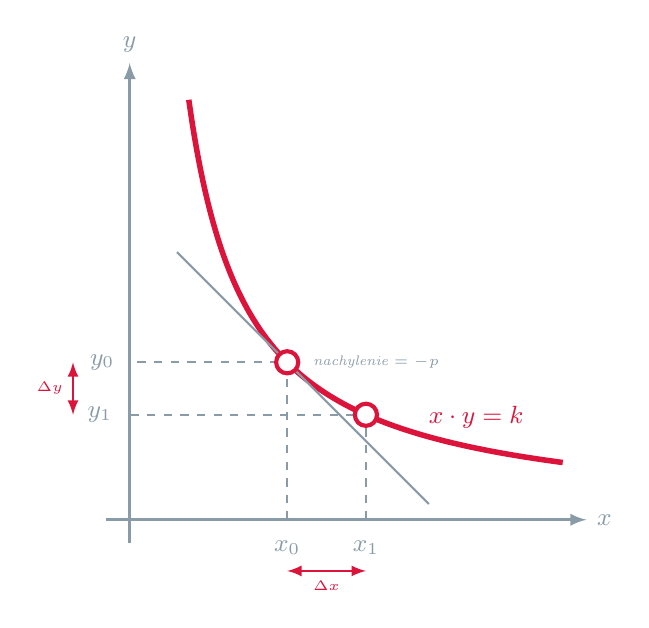
\begin{tikzpicture}[
        lbl/.style={font=\small\itshape, text=stplmuted},
      ]
      \draw[draw=stplmuted, -latex, line width=1pt]
        (-0.3,0) -- (5.8,0) node[right, lbl] {$x$};
      \draw[draw=stplmuted, -latex, line width=1pt]
        (0,-0.3) -- (0,5.8) node[above, lbl] {$y$};

      \draw[domain=0.75:5.5, smooth, samples=100,
            draw=stplred, line width=2pt]
        plot (\x, {4/\x});

      \node[font=\small\bfseries, text=stplred] at (4.4,1.3) {$x \cdot y = k$};

      % Dashed coordinate lines
      \draw[draw=stplmuted, dashed, line width=0.6pt] (2,0) -- (2,2) -- (0,2);

      % Axis tick labels
      \node[lbl] at (2,-0.35) {$x_0$};
      \node[lbl] at (-0.35,2) {$y_0$};

      % Second point after swap: x_1 = 3, y_1 = k/x_1 = 4/3
      \draw[draw=stplmuted, dashed, line width=0.6pt] (3,0) -- (3,{4/3}) -- (0,{4/3});
      \node[lbl] at (3,-0.35) {$x_1$};
      \node[lbl] at (-0.38,{4/3}) {$y_1$};

      % Delta annotations
      \draw[draw=stplred, latex-latex, line width=0.8pt] (2,-0.65) -- (3,-0.65)
        node[midway, below, font=\tiny\bfseries, text=stplred] {$\Delta x$};
      \draw[draw=stplred, latex-latex, line width=0.8pt] (-0.72,{4/3}) -- (-0.72,2)
        node[midway, left, font=\tiny\bfseries, text=stplred] {$\Delta y$};

      % Tangent at (2,2): y = -x + 4, slope = -1
      \draw[draw=stplmuted, line width=0.8pt] (0.6,3.4) -- (3.8,0.2)
        node[midway, above right, font=\tiny\itshape, text=stplmuted] {nachylenie $= -p$};

      % Points on curve — drawn last so they sit on top
      \filldraw[fill=stplwhite, draw=stplred, line width=1.5pt] (2,2) circle (4pt);
      \filldraw[fill=stplwhite, draw=stplred, line width=1.5pt] (3,{4/3}) circle (4pt);
    \end{tikzpicture}
  \end{center}
\end{frame}

\begin{frame}{Jak działa swap?}
  \begin{itemize}
    \item Użytkownik wpłaca $\Delta x$ tokenu A, otrzymuje $\Delta y$ tokenu B
    \item Nowe rezerwy są policzone tak, aby zachować $k = x \cdot y$
    \item Im większy swap względem puli, tym gorsza cena --- to \textbf{price impact}
  \end{itemize}
  \vspace{0.3cm}
  \begin{exampleblock}{Przykład: kupujemy 100 USDC za SOL}
    Pula: $x = 10$ SOL, $y = 1\,000$ USDC \quad $k = 10\,000$. \\
    Po cenie startowej (100 USDC/SOL) oczekujemy zapłacić 1 SOL.
    \[
      x' = \frac{k}{y - \Delta y} = \frac{10\,000}{900} \approx 11{,}11 \text{ SOL}
    \]
    Efektywna cena: $\approx 1{,}11$ SOL zamiast 1 SOL --- to price impact.
  \end{exampleblock}
\end{frame}

\begin{frame}{Impermanent Loss}
  \begin{itemize}
    \item IL jest tym większy, im bardziej cena odchyla się od ceny wejścia
    \item Przy powrocie ceny do poziomu wejścia --- IL znika (stąd \emph{impermanent})
    \item LP profituje gdy: \textbf{opłaty > IL}
    \item Strategia: pule stabilnych par (np.\ USDC/USDT) mają minimalne IL
  \end{itemize}
  \vspace{0.3cm}
  \begin{alertblock}{\textbf{Impermanent Loss (IL)}}
    Gdy cena tokenów zmienia się względem chwili wpłaty, wartość pozycji LP jest
    \emph{mniejsza} niż gdyby trzymać tokeny (HODL).
  \end{alertblock}
\end{frame}

\begin{frame}{Concentrated Liquidity}
  \begin{itemize}
    \item \textbf{Concentrated Liquidity Market Maker (CLMM)} --- LP wybiera \textbf{przedział cenowy} $[p_a,\, p_b]$, w którym działa
    \item Kapitał jest efektywniejszy --- więcej płynności tam, gdzie handel
    \item Wyższe opłaty przy trafnym wyborze zakresu
    \item Wyższe ryzyko IL przy wyjściu ceny z zakresu
  \end{itemize}
  \vspace{0.3cm}
  \begin{exampleblock}{Na Solanie}
    \textbf{Orca Whirlpools}, \textbf{Raydium CLMM} --- wiodące implementacje CLMM
  \end{exampleblock}
\end{frame}

% ================================================================
\section{Podsumowanie}

\begin{frame}{Podsumowanie}
  \begin{itemize}
    \item \textbf{DeFi} --- usługi finansowe bez pośrednika; token to saldo z regułami w kodzie
    \item \textbf{AMM} zastępuje order book proporcją rezerw --- duży swap kosztuje więcej
    \item \textbf{LP} dostarcza płynność i zarabia opłaty, ale wartość pozycji zależy od cen
    \item Drugi filar DeFi --- pożyczki --- w kolejnej lekcji
  \end{itemize}
\end{frame}

% ================================================================
\begin{frame}[plain]
  \begin{center}
    \vfill
    {\Huge\bfseries\color{stplwhite} gn}
    \vfill
  \end{center}
\end{frame}

\end{document}
